\chapter{Toolbox for \omen in \matlab (TOM)}

	\gls{TOM} was programmed to simulate spherical nanocrystals and to visualize the results of the simulations.
	Though we focused on spherical structures, the code is hold abstract and slim to make extending to other
	structures, such as nanowires, fairly easy.
	The main aim of \gls{TOM} is to offer \omen users a toolbox, which includes the following 3 main tasks:
	\begin{enumerate}
		\itemsep 0pt
		\item Automatization of the \omen simulation process \\
					When it comes to simulating \glspl{QD} with different parameters, users do not want to spend a lot
					of time on writing command files for OMEN by themselves and start each OMEN task via the shell, but 
					rather enter the main parameters into a \gls{GUI} and let \gls{TOM} do the rest (see section \ref{sec:RunSim}).
					This makes overnight simulations for large parameter sets possible.
		\item Overview of all simulations done in the past	\\
					All information respectively parameters of past simulations can be displayed in a \gls{GUI}. Exporting selected
					simulations and visualizing them is possible as well (see section \ref{sec:guiDB})
		\item Visualization of simulation data	\\
					All different kinds of plots are available within the toolbox, such as visualizing band gaps, wave functions or
					quantum dot structures (see section \ref{sec:plotting}).
	\end{enumerate}

	\section{Installing the Software}
		You can get a version of \gls{TOM} at the \gls{LNE} at {\sc ETH} Zurich. Copy the folder \lstinline{TOM} to any directory on your computer.
		Now it is necessary to define some paths. Open therefore \lstinline{TOM/System/initTOM.m} and change all fields, that are listed below.
		The field {\it root} contains the path, where the folder \lstinline{TOM} is saved. Equivalently change the fields OMEN and simulations. Note,
		that these paths do not have to direct to a subfolder or TOM, i.e. simulation data can be stored anywhere on the computer.
		\begin{lstlisting}
			config.root     	  = '/usr/home/TOM/';
			config.OMEN         = [config.root, 'OMEN_ethz-amd64'];
			config.vOMEN        = '04May2013';
			config.simulations  = [config.root, 'Simulations/'];
		\end{lstlisting}

	\section{Using a newer version of \omen}
		If you would like to use a newer version of \omen, please make the following changes. Open the \lstinline{TOM/System/initTOM.m} file
		and change \lstinline{config.vOMEN} to the date, when the \omen version you are using was released. Afterwards copy the new \omen executable
		to the path defines in \lstinline{config.OMEN}
		It might be possible, that simulations do not run with the new file, as the rights are not set to {\it executable}. In this case, right click on
		the executable, select properties and afterwards {\it Run as executable}. 
	
	
	%%%%%%%%%%%%%%%%%
	%   USING TOM   %
	%%%%%%%%%%%%%%%%%
	\section{Using TOM}
		\subsection{Basic concept}
			%BASIC CONCEPTS
				The {\bf first step} when you want to work with \gls{TOM} is its initiation. Therefore add the \software folder including subfolders to the \matlab path,
				type \lstinline{initTOM.m} in the command window and hit enter.
				
				Typing \lstinline{help TOM} will provide you with all available functionalities including a description how to use them. Another way to
				get help is by opening the \gls{TOM} manual, which can also be accessed via the help command or the menu lists in the \glspl{GUI}.
				
				Table \ref{tbl:functionParmeters} gives a quick overview of the most important function parameters, that are used regularly in the \gls{TOM} code.
			
				Parameters for the simulation are stored and passed as objects to functions of the class \textit{Qdot}, further referred to as \gls{QDO}. 
				The class provides properties for all parameters necessary for the simulation, as well as properties for administrative purposes, such as the 
				specific simulation folder. Parameters relating to the geometry are stored in an object of subclass \textit{Geometry}. Since more than one material 
				is possible, the geometry property is often an array of objects of class Geometry. 
				To instantiate a \gls{QDO}, one can call the constructor with no arguments, which will create an empty \gls{QDO}. Alternatively, a string with the material 
				name can be passed as an argument, in which case the new \gls{QDO} will be constructed based on parameters defined in an external file, located 
				in the folder \textit{Classes}.
				The class \textit{Qdot} provides some methods for basic displaying of some selected parameters, such as \textit{getSelParams}.\\\\
				\begin{EXAMPLE}
					Creating a \textit{Qdot} object based on default parameters and set the radius to 4
					\begin{lstlisting}[frame=none]
						myQdot = Qdot('CdS_CdSe');
						myQdot.geometry(2).radius = 4;
					\end{lstlisting}
				\end{EXAMPLE}
	
				\begin{table}[htbp]
					\centering
					\begin{tabular}{ll}
						DIR						&	Directory path														\\
						EDO						& Experimental data object									\\
						EDOA					& Array of experimental data objects				\\
						QDO						& Quantum dot object												\\
						QDOA					&	Array of quantum dot objects							\\
						propertyName	& Property name of an EDO or QDO						\\
						BGap					& Band Gap																	\\
						NMod					& Number of modes														\\
						NOrb					& Number of orbitals												\\
						band					& CB: Conduction band or VB: Valence Band		\\
						tol						& tolerance																	\\
					\end{tabular}
					\caption{Important function parameters}
					\label{tbl:functionParmeters}
				\end{table}
				
		% RUNNING A Simulation
		\subsection{Running a simulation} \label{sec:RunSim}
			Type gui\_simulate \index{gui\_simulate} in the \matlab command window and hit enter. The window as in figure \ref{fig:gui_simulate} will open.
			\begin{figure}[htbp]
				\centering
				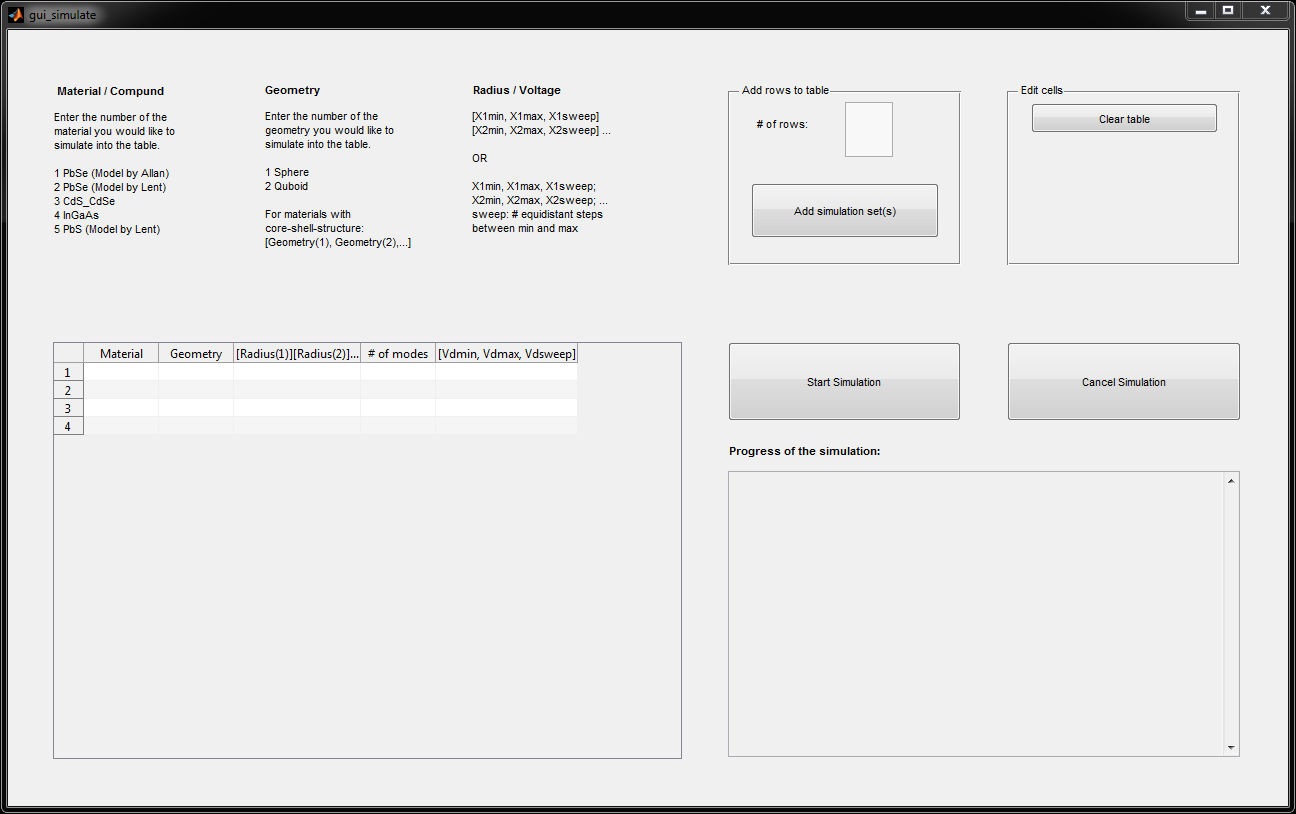
\includegraphics[width=0.8\textwidth]{Fig/Scrn_gui_simulate.png}
				\caption{The gui\_simualte window}
				\label{fig:gui_simulate}
			\end{figure}
			A simulation set is defined as one row of the table, i.e one material with all kinds of sweeps. You can add more simulation sets
			by using the {\it Add rows to the table} panel.
			It is possible to copy and paste single cells of the table using the appropriate short cuts of your \matlab default keyboard setup
			(\lstinline{CTRL+C & CTRL+V} Windows setting, \lstinline{ALT+W & CTRL+Y} Emacs setting).
			The columns are filled as follows:
			\begin{enumerate}
				\item Material		\\
							Enter the number for the material you would like to simulate, according to the {\it Material / Compound} list. \\
							\begin{tabular}{ll}
								{\it Material Name}\_lent		&	Simulations done with Tight binding parameters by Lent	\\
								{\it Material Name}\_allan	&	Simulations done with Tight binding parameters by Allan	\\
							\end{tabular}
				\item Geometry		\\
							Enter the number of the geometry given in the {\it Geometry} list. Very important in the case of materials with
							shells is, that you have to enter the geometry type of the core and the shell. The geometry types are separated	
							with a comma.
							\begin{EXAMPLE}
								For a spherical CdS-CdSe quantum dot the cell would look like this: 1, 1
							\end{EXAMPLE}
				\item Radius [$nm$]			\\
							The radius has to be entered in a specific way. The syntax is: 						\\
							\lstinline{[Rmin(1), Rmax(1), Rsweep(1)][Rmin(2), Rmax(2), Rsweep(2)]...} \\
							\newline
							\begin{tabular}{@{}ll}
								Rmin(i)		& smallest radius of the i\textsuperscript{th} material to be simulated		\\
								max(i)		& largest radius of the i\textsuperscript{th} material to be simulated		\\
								Rsweep(i)	& number of equidistant points between Rmin(i) \& Rmax(i)									\\
							\end{tabular}
							
							\begin{EXAMPLE}
								For the simulation of a single spherical PbS quantum dot with radius 3.5 nm you would enter: [3.5,3.5,1]
							\end{EXAMPLE}
				\item \# of modes	\\
							Enter a number of modes you would like to calculate.
				\item Electric field in units [$V/nm$]			\\
							The electric field sweep is entered in the same way as the radius. You find more information under the following remark.
				\item update\_bs\_target	\\
							For higher electric fields \omen cannot differentiate conduction and valence band, therefore the user has to make a guess
							where the band gap might be. \omen will then simulate the \# of modes around this given energy (bs\_target).
							If you would like to make use of this option enter 1 in the {\it update\_bs\_target} field otherwise 0.
							Please note, that if you choose 0, you will have to enter any numerical value (i.e. 0) in the {\it bs\_target} field as well, otherwise
							the \gls{GUI} cannot process the data.
				\item bs\_target [eV]	\\
							The energy value around which the energy levels are calculated.
				\item Permute	\\
							Enter 0, if the radii vectors should be combined element wise, i.e. first element of R(1) and R(2) give a simulation, second element
							of R(1) and R(2) give a simulation and so on. Each radius pair will be simulated with all possible electric fields specified.
							Selecting 1 will permute all possible radii with each other and all electric fields.
							\begin{EXAMPLE}
								For a spherical CdS-CdSe quantum dot the input cell would look like this: [1,4,4][5,6,2]
								 If you select Permute = 1, \software will calculate all possible permutations and generate therefore 8 quantum dots: \\
								\newline
								\begin{tabular}{@{}lcccccccc}
									Quantum dot					&	1	&	2	&	3	&	4 &	5	&	6	& 7	&	8	\\
									Core radius	in nm		&	1	& 1 & 2 & 2 & 3	& 3 & 4 & 4	\\
									Shell radius in nm	& 5	& 6 & 5 & 6 & 5 & 6 & 5 & 6	\\
								\end{tabular}
							\end{EXAMPLE}
							
							\begin{EXAMPLE}
								For a spherical CdS-CdSe quantum dot the input cell would look like this: [1,2,2][3,4,2]
								If you select Permute = 0, \software will combine elementwise the entries of the two vectors: \\
								\newline
								\begin{tabular}{@{}lcccccccc}
									Quantum dot					&	1	&	2	\\
									Core radius	in nm		&	1	& 2	\\
									Shell radius in nm	& 3	& 4	\\
								\end{tabular}
							\end{EXAMPLE}
			\end{enumerate}
			
			\begin{REMARK}[Vectors \& Matrices] \index{Vector}
				As the \matlab \gls{GUI}s do not accept vectors or matrices as it is known from the command window, the parameters
				have to be entered as a string and are converted to matrices later on.
				
				There are different ways how to enter the parameters. Use the one, that is the most clear for you.
				\begin{lstlisting}
               a,b,c,...,d                 or
              [a,b,c,...,d]                becomes a double vector

              V = [ a b c ... d]


              [a,b,c][d,e,f]...[g,h,j]     or
               a,b,c; d,e,f;...;g,h,j      or
              [a,b,c; d,e,f;...;g,h,j]     becomes a double matrix

              M = [ a b c
                    d e f
                    . . .
                    g h j ]

              where a,b,...,j are doubles as strings.
   			\end{lstlisting}
   			These input styles can be applied to column {\it Geometry}, {\it Radius} and {\it Voltage}.	\\
   			You can use as many spaces as you want in between. The first and the last brace are not necessary if only a vector is entered or if
   			rows are separated by semicolons.
			\end{REMARK}
			
			After entering all the necessary parameters proceed by clicking \lstinline{Start Simulation}. The {\it Progress of the simulation} panel will
			keep you informed about the warnings, wrong entered parameters and the current status of the simulation.
			

		% DISPLAY SIMULATION INFORMATION
		\subsection{Display simulation information} \label{sec:guiDB}
			There are two ways of displaying simulation information, either you can see the whole database \index{Database} (all simulations
			that are stored in the \lstinline{Simulations} folder) or only specific data, for example only PbS simulation data.
			
			\begin{REMARK}
				\software uses objects (called {\it qdotObj}) to store all important data of simulations such as the simulation parameters, date of simulation etc.
				(for further see information section \ref{sec:SoftwareStructure}). All operations are done using these objects. If you would like to display only
				certain simulation data, you would need an {\it qdotObj} array, called \gls{QDOA}. How to create such an array please read section \ref{sec:addTools}.
			\end{REMARK}
			
			Displaying the whole database can be done by typing \lstinline{gui_db} \index{gui\_db} into the \matlab command window. A window as in figure
			\ref{fig:gui_database} will appear showing all parameters and technical information of each simulation. Please note, that according to the size
			of the database, it might take some seconds to load all data.
			If you only want to display a set of simulation data, you can also call \lstinline{gui_db(QDOA)}.
			
			\begin{figure}[htbp]
				\centering
				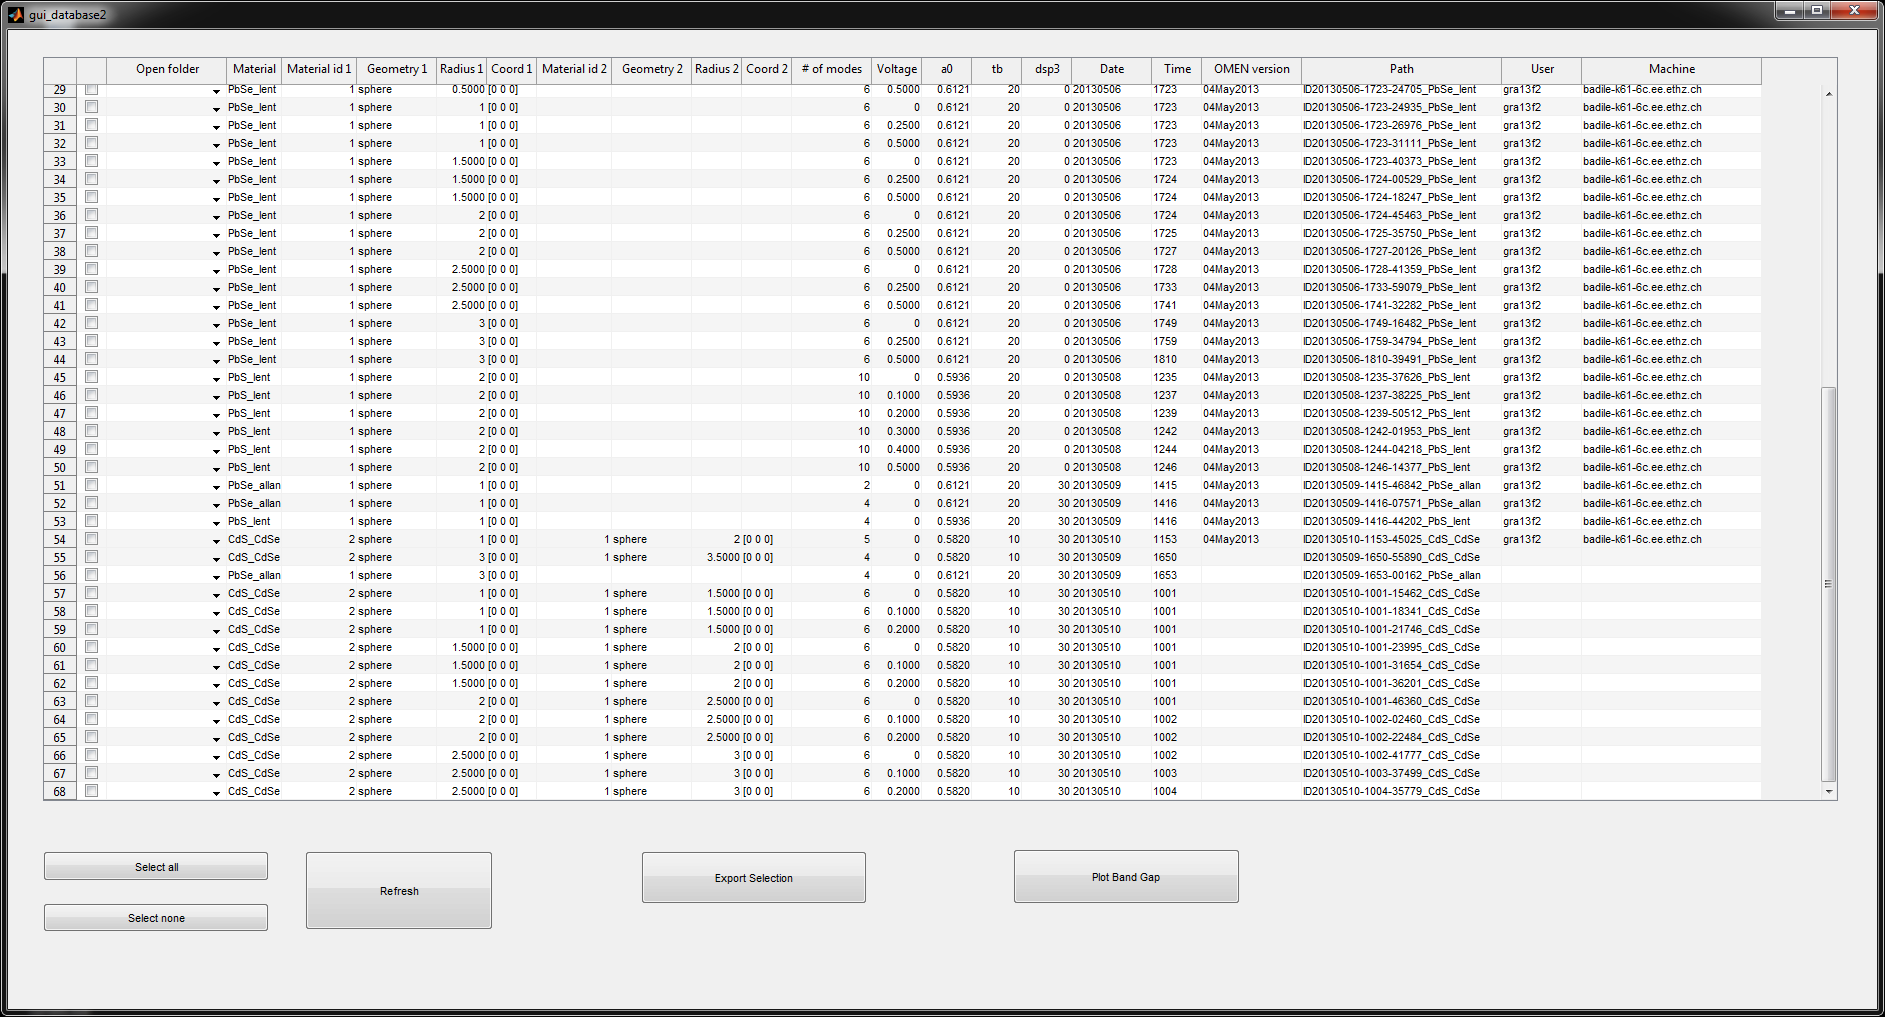
\includegraphics[width=\textwidth]{Fig/Scrn_gui_database.png}
				\caption{The gui\_database window}
				\label{fig:gui_database}
			\end{figure}
						
			Within the \gls{GUI} you can sort the simulations with the column header, select simulations and let them plot, open the directory of a simulation or 
			even export a selection, which is available as an \gls{QDOA} in the main workspace entitled {\it ExportedDB}.

		\subsection{Plotting} \label{sec:plotting}
			%PLOTTING
			Here follows a short description of functions, which can be used for basic visualization of the data obtained by the OMEN simulation. 
			For a more detailed description, please refer to the code.
			\textit{Note:}
			These functions are based on the directory structure created by the simulation function \lstinline{simAll.m}, i.e. to work properly, the simulation data, 
			as well as the corresponding \gls{QDO} must be located in their own folder, with the folder name specified in QDO.path property.
			
			\subsubsection{Plotting the wavefunction}
				%PLOTTING WAVEFUNCTIONS
				These functions all take an array of \textit{Qdot} objects (QDOA) as an input. Additionally, the number of eigenmodes to be displayed has to be specified, 
				as well as the band (conduction or valence band). The visualization will then be done for every one these objects, and for all specified eigenmodes.\\ \\
				\lstinline{function plotEV3D(QDOA, band, NMod) }\\\\
				Plot the atoms of the quantum dot, their color indicating the probability density of an electron or hole. Red corresponds to high, blue to low probability.\\ \\
				\lstinline{function plotEV3DcrossSection(QDOA, NMod) }\\\\
				This function produces similar plots to the above, but it plots two cross sections of the quantum dot, for valence and conduction band respectively, 
				in one window.\\\\
				\lstinline{function plotEV3Dmax(QDOA, band, probLim, NMod)}\\\\
				Again very similar to the \textit{plotEV3D}, but the color code is simplified. The atoms with very high probability densities are red, the ones with high 
				probability yellow, the rest transparent. The color is determined in the following way: The sum of the probabilities of all red atoms is smaller than a 
				probability value specified in \textit{probLim}. An analogous argument is applied for the yellow marked atoms.\\
				This function makes it a lot easier to see how the wavefunction roughly looks like and changes from one mode to the next.\\\\
				\lstinline{function plotEVAlongAxis(QDOA, propertyName, startPoint, direction, plotGrid,                           tolerance, NMod, band)}\\\\
				Plot the probability density along an arbitrary axis through the crystal. The data for all elements of QDOA is plotted in the same plot, thus making it easier
				 to compare quantum dots with different parameters. The axis is specified through \textit{startPoint} and \textit{direction}, including a tolerance, which is 
				 the maximum distance which an atom can deviate from the specified line. Depending on the direction, the tolerance has to be adjusted to include 
				 a sufficient number of atoms. To check this, it is useful to specify the input argument gridPlot, which will plot the atoms, the chosen axis, and highlight 
				 the atoms on the line in red. However, this function is probably only suitable for large quantum dots. Furthermore an averaging over neighboring atoms 
				 would be recommendable.	\newpage
				\lstinline{function compareEV(QDOA, band, NMod, tol, propertyName, showGrid)}\\\\
				Plots the same as \textit{plotEVAlongAxis}, but for three different directions (x,y,z axis), and arranges them in subplots in one figure.
				
				\subsubsection{Plotting energies}
				%PLOTTING ENERGY LEVELS
				\lstinline{function plotBandGap(QDOA)} \\\\
    		Plots the band gaps of a \gls{QDOA} in dependence of radius and applied voltage. Calling the function without an input argument,
    		will create plots for the whole database.\\\\
    		
    		\lstinline{function plotEnergyLevels(QDOA)}\\\\
    		Plots all simulated energy levels of an array of \glspl{QDO} and highlighting the band gap.\\\\
    		
    		\lstinline{function plotVoltBandGap(QDOA)}\\\\
    		Plots the band gap against voltage for a constant radius. The \glspl{QDO} have to have the same radius/radii.
				
				
		\subsection{Additional tools} \label{sec:addTools}
			%DATABASE
			In order to know which parameter sets already have been simulated, there are some useful tools, which can be found in the folder \textit{Functions/
			QdotUtils}. The basic principle is to get all all parameters which were simulated, which can then be displayed in the GUI, filtered, deleted and so on.
			
			\subsubsection{Getting the parameters from all simulations}
				\lstinline{function getQDOA()}\\\\
				This is done by loading the QDOs of all performed simulations from their folders, and storing them in a QDOA.
				 
			\subsubsection{Filtering}
				%FILTERING
				\lstinline{function filtered = filterQDOA(QDOA, propertyName, value, mode, tol)}\\\\
				The filtering can be applied to any QDOA, and returns a subset of this array, matching specified criteria. The argument \textit{propertyName} 
				specifies the \textit{Qdot} property which is compared to \textit{value}. The filter criteria are specified by selecting a mode of filtering. 
				The following filtering modes are available:\\
				\begin{itemize}
					\item the property exactly matches \textit{value}.
					\item the property lies within a range of values, specified by a vector: \textit{value} = [min max]
					\item the property approximately matches \textit{value}. For numeric properties this is specified using a tolerance. For string properties the \textit{value} 
					should be a substring of the property.
					\item filter for a constant difference between two properties. The property names are specified in a cell array: \textit{propertyName} 
					= \{\textit{propertyName1, propertyName2}\}
					\item filter for a constant ratio between two properties.
				\end{itemize}
				The last two modes are especially interesting for selecting \glspl{QDO} with two or more materials, to find the objects with a specified shell-thickness.\\
				\newpage
				\begin{EXAMPLE}
					Filter for QDOs with different properties
					\begin{itemize}
					\item[-] radius = 3.5nm
					\item[-] constant difference of 0.7nm (with a tolerance of +/- 10\%) between radius of material 1 and radius of material 2.
					\item[-] material containing Pb.
					\end{itemize}
					\begin{lstlisting}[frame = none]
					myQDOA = getQDOA;
					selection1=filterQDOA(myQDOA,'geometry(1).radius',3.5,1,0);
					selection2=filterQDOA(myQDOA, {'geometry(1).radius','geometry(2).radius'},0.7,4,0.1);
					selection3=filterQDOA(myQDOA,'mat_name','Pb',2,0); \end{lstlisting}
				\end{EXAMPLE}
			 
	
	%%%%%%%%%%%%%%%%%%%%%%%
	%   MAINTAINING TOM   %
	%%%%%%%%%%%%%%%%%%%%%%%
	\section{Maintaining \software}
		\subsection{General Structure} \label{sec:SoftwareStructure}
			\gls{TOM} stores all files of one simulation in a folder. To avoid conflicts in the the folder names are bijective. They
			have the following form \lstinline{IDyyyymmdd-hhmm-ssfff_MATNAME}. The name contains the date and time (including milliseconds)
			when the simulation was started as well as the name of the material, that is simulated. Figure \ref{dir:SimSetTree} illustrates
			the structure of a simulation folder. Note, that if you simulate with parameter \lstinline{update_bs_target = 1}, \omen will
			not create files for valence and conduction band, but rather write all eigenenergies into \lstinline{VB_E_0_0.dat} or
			\lstinline{CB_E_0_0.dat}.
			If you would like to make changes in \gls{TOM} or add new structures, such as nanowires, it is useful to get familiar with the
			workflow of the the software. Figure \ref{fig:Workflow} shows the function calls during the process.
		
			\begin{figure}
				\centering
				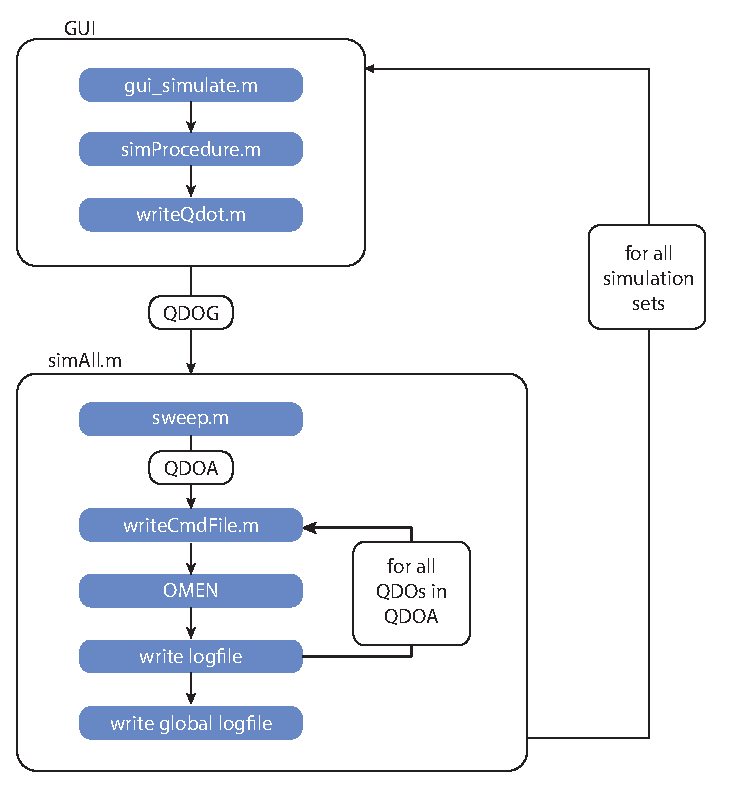
\includegraphics[width=0.75\textwidth]{Fig/workflow.eps}
				\caption{Workflow of the simulation procedure.}
				\label{fig:Workflow}
			\end{figure}
		
			\begin{figure}[htbp]
				\begin{minipage}[b]{0.59\textwidth}
				% Creates a directory structure figure
				\dirtree{%
				.1 /root.
					.2 TOM.
						.3 Classes.
						.3 DataUtils.
						.3 GUI.
						.3 Plotting.
						.3 SimProcedure.
						.3 System.
					.2 OMEN.
						.3 OMEN executables.
					.2 Simulations.
						.3 ID*.
						.3 \vdots.
						.3 log.
				}
				\caption{The \software structure by default}
				\label{dir:ToolboxTree}
			\end{minipage}
			\hfill
			\begin{minipage}[b]{0.39\textwidth}
			\dirtree{%
			.1 ID*.
				.2 CB\_E\_0\_0.dat.
				.2 CB\_V\_0\_0.dat.
				.2 H\_0.dat.
				.2 Layer\_Matrix.dat.
				.2 qdot\_cmd.
				.2 qdotObj.mat.
				.2 simlog\_{\it yyyymmdd\_hhmm\_ssfff}.
				.2 VB\_E\_0\_0.dat.
				.2 VB\_V\_0\_0.dat.
			}
			\caption{Structure of a simulation set}
			\label{dir:SimSetTree}
			\end{minipage}
			\end{figure}
			
			\subsection{Simulation}
				% SIMULATION
				The simulation parameters from the GUI are passed to the functions which will then start the simulation with OMEN.
				The parameters are stored in QDOs. Since it is often desirable to simulate over a range of parameters, some parameters 
				(i.e. the radii and e-field) are at this stage not scalars, but a vectors, containing starting value, end value and number of steps in between. 
				Such a generic \gls{QDO},  is further referred to as \gls{QDOG}.
				\\\\
				The \gls{QDOG} is passed to the function \lstinline{simAll.m}, which will simulate all desired parameter combinations, by performing the following steps:
				\begin{itemize}
					\item An array of QDOs (QDOA) with all combinations of the parameter is created in the function \lstinline{sweep.m} from QDOG. 
					Supported sweep parameters are radius and electric field. This could easily be extended to other parameters by modifying the function \lstinline{sweep.m}.
					\item The elements in the QDOA are then simulated one after the other, and all data saved in seperate folders, called ID\lstinline{timestamp\material}: 
					\item The OMEN command-file \lstinline{qdot\cmd} is written, using the function \lstinline{writeCmdFile.m}.
					\item The OMEN simulation will be started using the MATLAB function \lstinline{unix}, which calls the operating system to execute the specified command.
					\item A logfile is written, recording the duration and the success of the simulation as well as the console output of OMEN. The success of the simulation
					is checked by inspecting whether the desired files were created.
				\end{itemize}
				After the simulation of all elements in the \gls{QDOA}, an additional logfile is written, and saved in the folder \lstinline{log}. It gives information about the 
				success of all simulations, and thus provides an easy way to check if and which simulations failed.
				\\\\
				Returned to the calling function is the \gls{QDOA} as well as a vector indicating the success of every simulation.
				\\\\
				Note that it is not strictly necessary to start the simulations using the GUI. The \gls{QDOG} containing the desired parameters can also be created with 
				standard MATLAB syntax, and passed subsequently to the function \lstinline{simAll.m}, as is shown in the following example.\\
				\\
				\begin{EXAMPLE} Simulate PbS  quantum dots with radii 1.5, 2, 2.5, 3nm. 
					\begin{lstlisting}[frame = none]
						myQdot = Qdot('PbS_lent');
						myQdot.geometry.radius = [1.5 3 4]; 
						simAll(myQdot);\end{lstlisting}
				\end{EXAMPLE}
					
	\section{Q \& A}
		\paragraph{Why is opening gui\_db is not possible?} It might be that there are failed simulations in the
		database. Please delete the according folders and try again.
		
		\paragraph{How can I stop the simulation?} \matlab is blocked during
			the time it has send a command to the shell. You might have to abort the process by pushing \lstinline{CTRL+C}
			a couple of times.
		
		\paragraph{Why does the simulation not start?}
			You might have to make to set up the right for \omen to execute: Tick 'Run as ' after right clicking
			the \omen executable and selecting properties.